\section{Experimental Analysis}
\label{sec:evaluations}

In this section, we discuss the experimental analysis of our design by describing the experimental methodology and comparing our system to existing LDPC decoders in solution quality, throughput, and energy consumption. 
These decoders can be implemented using GPUs, FPGAs, or as ASICs and are often 
explicitly designed to a particular code. We chose 3 implementations representating 
the state of the art ASIC decoders for 5G standards to compare against.

Behavioral simulation of our LDPC decoder's is done by solving Eq.~\ref{eqn:rim_node_simplifed}, 
using MATLAB's nonstiff, single step, 5th-order differential solver (ode45). Circuit parameters are 
obtained using Cadence with 45nm Generic Process Design Kit (GPDK045). 
We also ran a state-of-the-art variant~\cite{Isakov}  of 
Simulated Annealing to obtain solution quality for LDPC decoding using the traditional
QUBO formulation.

%which shows how the capacitor's voltage representing each node changes over time. $J_{ij}$ represents the effective conductance of the coupling with the parity equations. ${J_b}_i$ represents the bias conductance, ${v_b}_i$ represents the bias voltage. %and $v_i$ represents the current voltage on the node.



\begin{comment}
    

\subsection{Benchmarks and Metrics}

They are many standards defining LDPC codes for different applications. Most recently, the LDPC code has been standardized for wireless enhanced-mobile broad-band (eMBB) communication in 5G new radio (NR) by the 3-generation partnership project (3GPP). We use the LDPC codes defined by this standard as our benchmarks to compare the solution quality of different algorithms.

\begin{figure}[htp]
    \centerline{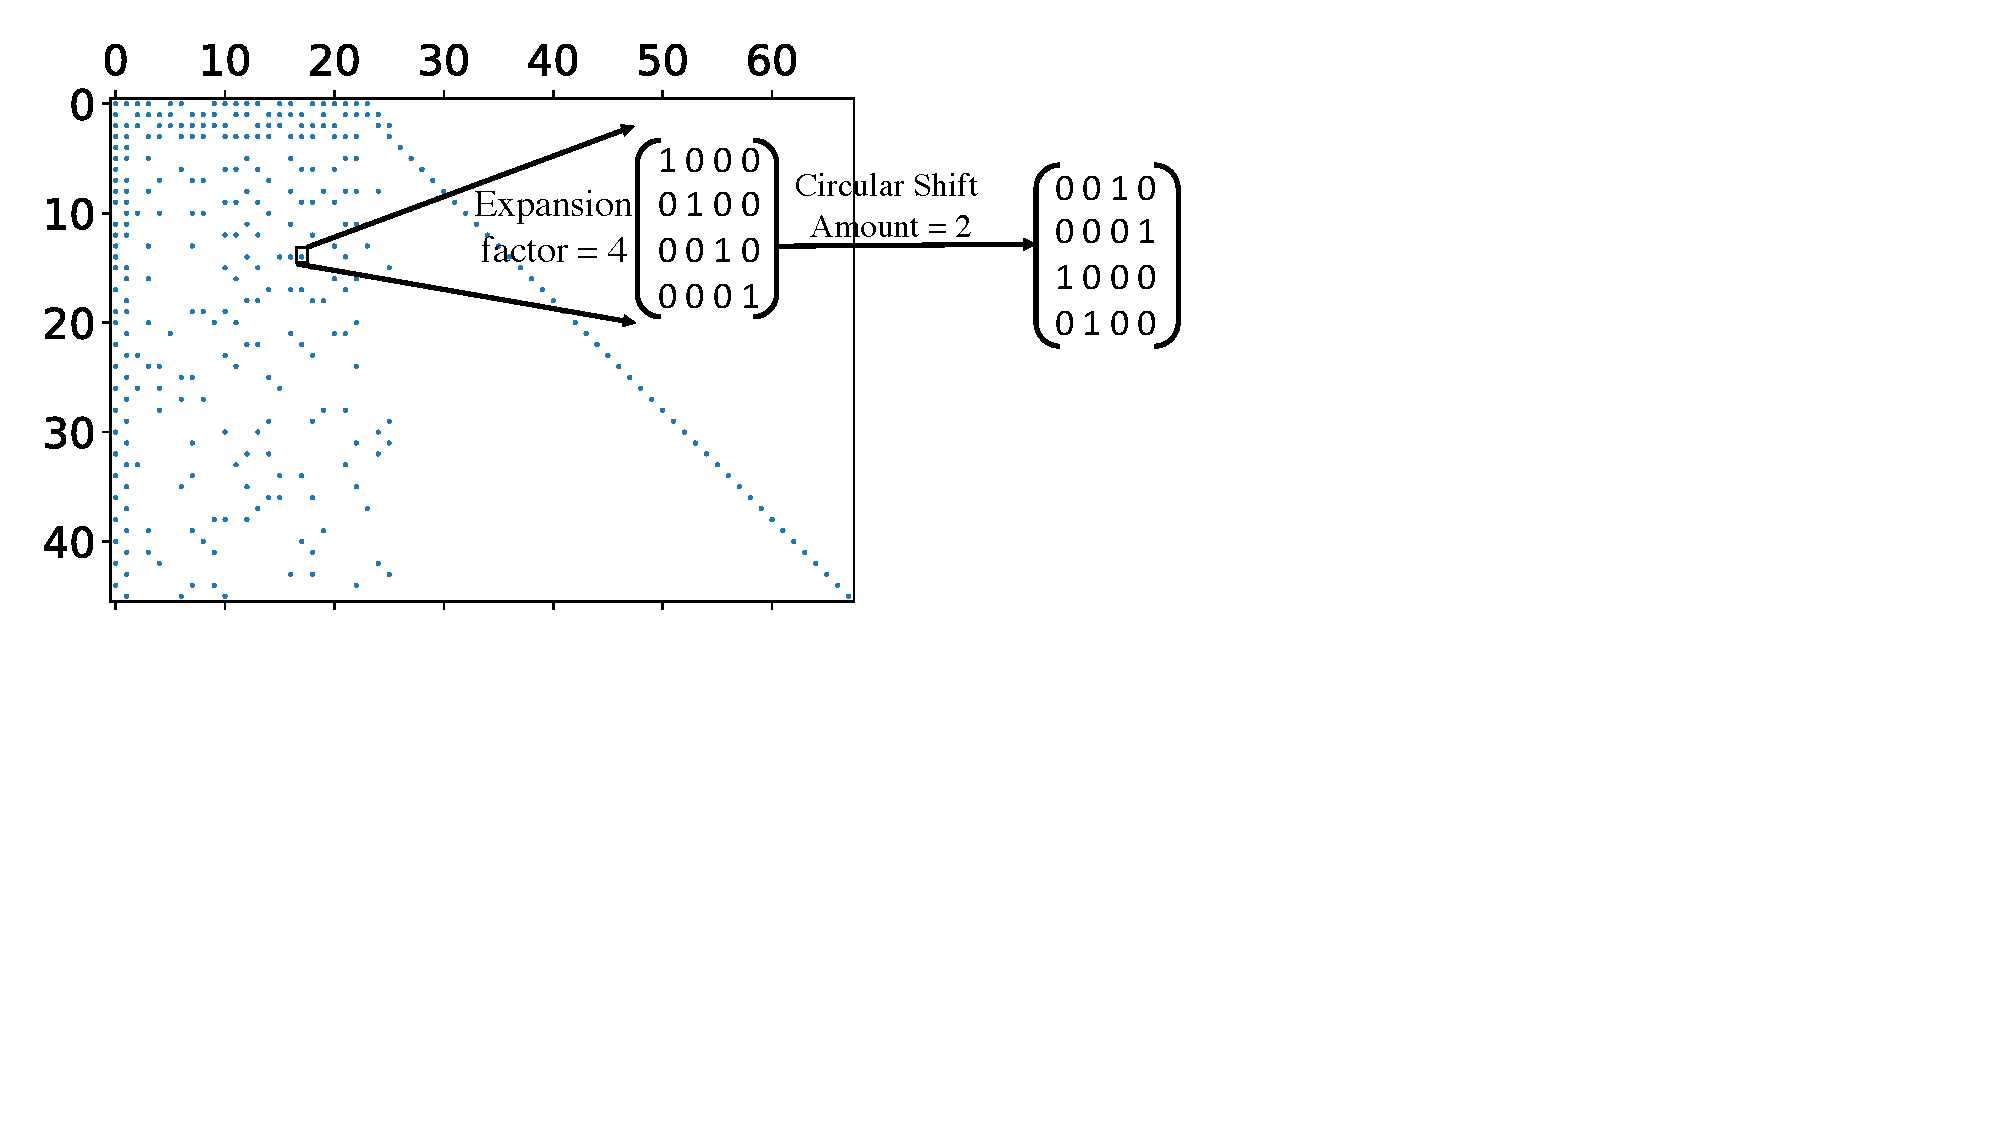
\includegraphics[width=0.47\textwidth]{FIGS/circular_shift.pdf}}
    \caption{Structure of 5G-NR standard base graph 1. Each blue dot represents a nonzero element which will be replaced by a circular identity matrix based on the expansion factor as shown.}
    \label{fig:5g-nr}
\end{figure}

\subsubsection{5G-NR standard} \label{sec:5g_nr_standard}
 The 5G standard describes two base-graph (BG) matrices: BG1 and BG2, which are used to construct a parity check matrix. Figure~\ref{fig:5g-nr} shows the structure of BG1. The blue dots in the figure~\ref{fig:5g-nr} show nonzero elements of the matrix. It has 46 rows and 68 columns, and the BG2 matrix has 42 rows and 52 columns. Rows in the base graphs describe parity check equations. By default, BG1 generates an LDPC code with a rate equal to $1/3$, and BG2 generates an LDPC code with a rate equal to $1/5$. Based on the required rate, we chose the base graph. 

Once the base graph is chosen, each zero entry is replaced with a $Z \times Z$ all-zero matrix. Each nonzero entry is replaced with a $Z \times Z $ circular shifted identity matrix. $Z$ is called an expansion factor. The amount of circular shift depends on the value of the nonzero element. The values of the nonzero elements range from 0 to z. If the value is 0, replace the element with the $Z \times Z$ identity matrix; otherwise, circularly shift the identity matrix based on the value. In figure ~\ref{fig:5g-nr} an example with an expansion factor of 4 and the circular shift amount of 2 is shown. The 5G-NR standard allows different discrete expansion factors ranging from 2 to 384. For any further details please refer to the following paper~\cite{bae2019overview}.

\subsubsection{Metrics}

To compare the solution quality of different algorithms, we use a metric called Bit Error Rate (BER). It defines the probability of a bit being erroneous; mathematically, it is defined as the ratio of the number of error bits by the total number of bits. The number of error bits is equal to the Hamming distance between the decoded and original message. Lower is better.

%The LDPC decoders are designed for different standards based on other design principles using alien technology. So we decided to use $Gbits/sec/Watt$ as the final figure of merit for comparison among different LDPC decoders

%\subsection{Architectural details for 5G-NR standards}\label{sec:5g-nr}
\end{comment}



%\subsection{Comparison with existing LDPC decoders}

\begin{comment}
\begin{table*}[htb]
\centering
\caption{comparison of hybrid LDPC decoder with existing decoders}
\label{table:comparision}
%\resizebox{\columnwidth}{!}
{
%\setlength{\tabcolsep}{4pt}
\begin{tabular}{|c|c|c|c|c|c|c|} 
\hline
\bf {Design\textbackslash Decoder} & \thead{~\cite{schlafer2013new}}  & \thead{~\cite{lin202133}} & \thead{~\cite{cheng2014fully}}   & \thead {~\cite{lee2022multi}}  & \thead{~\cite{thi2021low}} & \thead{this work}\\  
\hline\hline

CMOS Technology  &   65nm LVT  & 28nm & 90nm   & 65nm  & 65nm & 45nm\\ 
\hline
Standard        &  IEEE802.11ad   & 5G-NR   & -    &5G-NR & 5G-NR & 5G-NR \\ 
\hline
Decoding Algorithm & Min-Sum & \thead{ Normalized\\Min-Sum}   &  \thead{ Normalized\\Min-Sum}  & \thead{ offset\\Min-Sum} & \thead{Combined \\ Min-Sum} & \thead{hybrid \\ Ising model}  \\
\hline
Block size         &  672  &  \thead{all cases of 5G}  & 2048 & \thead{all cases of 5G} & 3808 & \thead{all cases of 5G} \\
\hline
\thead{Decoding Latency \\(iterations or annealing time) }  &  10 & 5 &  9 & 3 &10 & 0.22 $\mu sec$\\
\hline
Max Throughput (GBs/sec) & 160.8 & 6.7  & 45.09  & 21.78 &3.04 & 118.6 \\
\hline
Max Power (mW)    & 5360 & 232 & 1110 & 413 & 259 & 1566 \\
\hline
Area ($mm^2$) &   12.09  & 1.97 & 9.6 & 5.74 & 1.49 & 33\\
\hline
Energy (pJ/bit)  & 36.1 & 145  & 20.33  & 94.89 & 85.2& 13.14\\

%\hline
%Gbits/Sec/$mm^2$  & 13.30 & 3.4  & 4.7  & 3.82 & 2.04& -\\
%\hline

\hline
\end{tabular}
}
\end{table*} 
\end{comment}

\subsection{Comparison with existing LDPC decoders}
\begin{comment}
\begin{table*}[htb]
\centering
\caption{comparison of hybrid LDPC decoder with existing decoders}
\label{table:comparision}
%\resizebox{\columnwidth}{!}
{
%\setlength{\tabcolsep}{4pt}
\begin{tabular}{|c|c|c|c|c|c|} 
\hline
\bf {Design\textbackslash Decoder} & \thead{~\cite{schlafer2013new}}  & \thead{~\cite{lin202133}}   & \thead {~\cite{lee2022multi}}  & \thead{~\cite{thi2021low}} & \thead{this work}\\  
\hline\hline

CMOS Technology  &   65nm LVT  & 28nm   & 65nm  & 65nm & 45nm\\ 
\hline
Standard        &  IEEE802.11ad   & 5G-NR & 5G-NR & 5G-NR & 5G-NR \\ 
\hline
Decoding Algorithm & Min-Sum & \thead{ Normalized\\Min-Sum}   &  \thead{ offset\\Min-Sum} & \thead{Combined \\ Min-Sum} & \thead{hybrid \\ Ising model}  \\
\hline
Block size         &  672  &  \thead{all cases of 5G}  & \thead{all cases of 5G} & 3808 & 1088 \\
\hline
\thead{Decoding Latency per iteration\\ (nsec)} &  4  & 787 & 1530  & 125.33  & 220  \\
\hline
\thead{Max Throughput per iteration \\(GBs/sec)} & 160.8 & 33.2  & 17.06 & 30.38 & 4 \\
\hline
Max Power (mW)    & 5360 & 232  & 413 & 259 & 6.59 \\
\hline
Area ($mm^2$) &   12.09  & 1.97  & 5.74 & 1.49 & - \\
\hline
Energy (pJ/bit) per iteration  & 36.1 & 29  & 24.2 & 8.52 & 1.33\\
\hline
\thead{BER @ SNR 3 \\ exp\_factor = 16 \\ bit width =8bits }  &  5.69E-02 & \red{3.67E-02}  & 3.67E-02 & \red{3.67E-02} & 1.61E-02\\
\hline
\end{tabular}
}
\end{table*}

\todo{block size must be the same, increase either area or latency to compensate for the block size, equation}

\end{comment}

\begin{table}[htb]
\centering
\caption{Comparison of the proposed LDPC decoder with existing decoders, all parameters are adjusted to implement highest expansion factor}


%\donotshow{
%}

\label{table:comparision}
\resizebox{\columnwidth}{!}{
\setlength{\tabcolsep}{4pt}
\begin{tabular}{|c|c|c|c|c|} 
\hline
\bf {Design\textbackslash Decoder}  & \thead{~\cite{lin202133}}   & \thead {~\cite{lee2022multi}}  & \thead{~\cite{thi2021low}} & \thead{this work}\\  
\hline\hline

CMOS Technology    & 28nm   & 65nm  & 65nm & 45nm\\ 
\hline
Standard          & 5G-NR & 5G-NR & 5G-NR & 5G-NR \\ 
\hline
Decoding approach & \thead{ Normalized\\Min-Sum}   &  \thead{ offset\\Min-Sum \\ (OMS)} & \thead{Combined \\ Min-Sum} & \thead{Augmented \\ Ising machine}  \\
\hline
Block size         &  26112 & 26112 & 3808 (26112$^*)$  & 26112 \\
\hline
\thead{Decoding Latency per iteration\\ (nsec)}  & 787 & 1530  & 125.33 (860$^*)$  & 320  \\
\hline
\thead{Max Throughput per iteration \\(Gbs/sec)}  & 33.2  & 17.06 & 30.38 & 81.6 \\
\hline
Max Power (mW)     & 232  & 413 & 259 & 158.24 \\
\hline
Area ($mm^2$)  & 1.97  & 5.74 &  1.49 & 5.44 \\
\hline
Energy (pJ/bit) per iteration   & 29  & 24.2 & 8.52 & 1.94\\
\hline
quantization   & 5  & 8  & 4 & 8\\
\hline
%\thead{BER \\  SNR = 2 \\exp\_factor = 64}   & - & - & - &-\\
%\hline
\end{tabular}
}
\footnotesize *Latency scaled for direct comparison with other designs.
%\todo{change xxx and yyy to original paper numbers}
\end{table}


\subsubsection {Comparison with ASIC LDPC decoders}
Table~\ref{table:comparision} shows a detailed comparison of our work with existing ASIC LDPC decoders. 
The decoders are designed for 5G standards.~\cite{lin202133},~\cite{lee2022multi} support all the LDPC codes described by the 5G standards, whereas~\cite{thi2021low} is designed for a particular code created by a specific expansion factor.~\cite{thi2021low} reported their parameters for a decoder intended for an expansion factor of 56. We have modified its decoding latency to represent the decoder designed for an expansion factor of 384 by keeping area and power constant—all the other parameters are directly obtained from the corresponding papers. The table shows that our physical computation-based decoder consumes 4.4 times less energy per bit than the state of the art. Finally, earlier work using Ising machine for LDPC decoding achieves only 21Mb/s~\cite{kasi2020towards}.

\begin{comment}
These ASIC LDPC decoders use different standards and different technologies. They are designed by hard-wiring different variations of the Min-Sum algorithm. 

We designed our BRIM-based LDPC decoder to implement all the codes defined by the 5G-NR standards. The maximum expansion factor allowed by 5G standards is 384, and the maximum number of columns and rows are 68 and 46, respectively. If we construct a code using these factors, it results in a parity check matrix of size $17664 \times 26112$. Suppose we choose a naive design to accommodate this parity check matrix. In that case, we require a system with $26112$ nodes and $17664 \times 26112 = 461242368$ parity units. As described in section~\ref{sec:5g_nr_standard}, the nonzero elements are replaced by a circular shift identity matrix. So even if we consider all $46 \times 68$ matrix to be nonzeros, maximum, we require $46 \times 68\times 384=1024512$ parity units. So to reduce the space and energy, we designed our system with $26112$ rows but $46$ columns. Each row would represent a node, and each column would represent $384$ parity equations. To represent these parity equations, we need $384\times 2$ different wires in each column. If we layout our chip with 45nm technology using four metal layers, 27 $\mu$m wide~\footnote{According to the following paper~\cite{sicard2011introducing} in 45nm technology in metal layers, 1 to 4, the wire width is 60nm, and the space between wires is 80nm}.
If we consider the parity units to be $1\mu$m in length, then the total area of the chip would be 33$mm^2$ approximately. The total annealing time to decode a code word is $0.22 \mu s$, which results in a throughput of 118.6 Gbits/sec. We calculated the maximum power consumed by this system to be 158.24 mW~\footnote{There are 316 nonzero elements in base graph 1. So only $316X384 = 121344$ parity units will be active for a parity check matrix constructed using an expansion factor of 384.}. Hence from this design, we can at least achieve an order of magnitude reduction in energy consumption per bit when compared to other state of the art designs.

\begin{figure}[htbp]
    \centering
    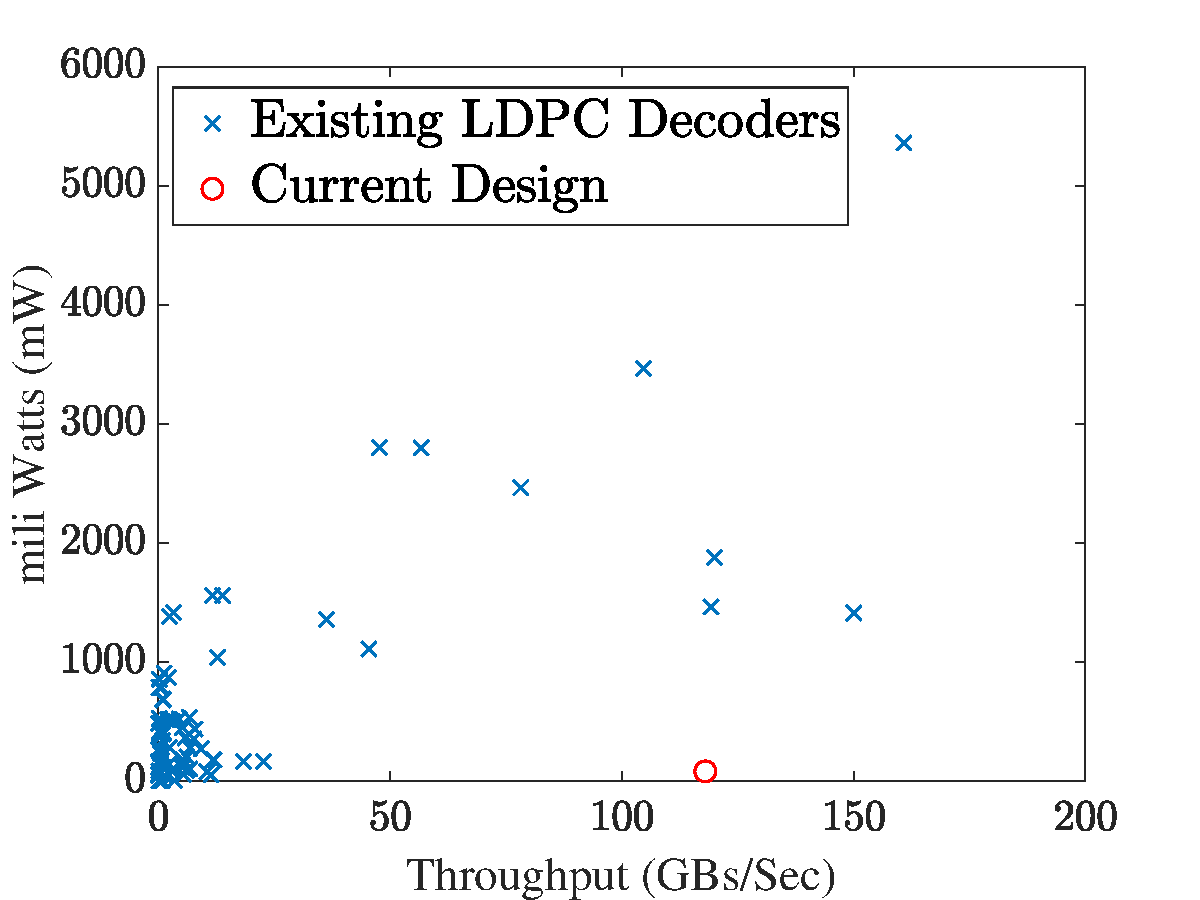
\includegraphics[width=0.45\textwidth]{FIGS/perfomance_ldpc.pdf}
    \caption{Performance vs Power Consumption of various LDPC decoders implemented in literature}
    \label{fig:ldpc_results}
\end{figure}

Figure~\ref{fig:ldpc_results} shows the graph of throughput vs power consumption of ASIC LDPC decoders. The graph is obtained from the following survey papers ~\cite{kingston2021certain,maunder2016survey}. \blue{Even in this graph, all the LDPC decoders are designed with different technology and for different standards. The graph shows that power consumption grows exponentially with the growth in throughput. In our design, parity units are responsible for most power consumption. They grow linear to the expansion factor. Hence, using our design, we could achieve linear growth in power consumption with throughput.}
\end{comment}
%\subsubsection{Comparison with existing Ising machines}

%As discussed in the following section~\ref{?} after conversion, the problem size of 5G-NR LDPC code with an expansion factor of 384 increases to \blue{48769} spins. 

%\todo{need to write}
\begin{comment}

\subsection{Comparison of solution quality of different algorithms }\label{sec:solution_quality}

One thousand messages were encoded using different LDPC codes to obtain the solution quality. These codes were constructed using the 5G-NR standard's base graph 1 with varying factors of expansion. The encoded messages were then modulated using BPSK modulation. The noise was added to the modulated signals based on the signal-to-noise ratio (SNR). These corrupted signals were used to test the different algorithms for solution quality. 

In Figure~\ref{fig:ber} labels 1 to 10 represent the maximum number of iterations used for decoding in the Min-Sum algorithm. QUBO represents the decoding of LDPC codes using QUBO formulation. Modified QUBO represents LDPC decoding using the proposed design. Both modified QUBO and QUBO were annealed for 0.22$\mu$s to obtain BER. The Min-sum algorithm is deterministic, whereas QUBO and modified QUBO are probabilistic. So, we used a different metric called Expected BER to estimate the solution quality. Each message (or instance) was annealed 100 times with random initializations. Each different anneal gives us a different solution. We find the distinct solutions in these different anneals and rank them according to their Ising energies. Considering this order static, the \textit{expected} Bit Error rate (E(BER($N_a$)))~\cite{kim2019leveraging} for each instance is calculated using the formula~\ref{eqn:expected_ber}.

%Figure ~\ref{fig:ber} shows the Bit Error Rate (BER) of different algorithms at different SNR values. The titles of each graph show the expansion factor used for creating the LDPC codes.

\begin{equation}\label{eqn:expected_ber}
\begin{split}
E(BER(N_a)) = \sum_{k=1}^{L} \left[ (\sum_{r=k}^{L} P_I(r))^{N_a} -  (\sum_{r=k+1}^{L} P_I(r))^{N_a}\right] \\ F_I(k)/N     
\end{split}
\end{equation}

 

where N is the number of bits in the message, L is the number of unique solutions obtained by different anneals, r is the rank index of each solution, $P_I(r)$ is the probability of obtaining the $r_{th}$ solution, and $F_I$ is the number of bit errors in the $k^{th}$ solution, relative to the ground truth. The average of 1000 different expected BER is reported as the final Bit Error rate for each SNR. As shown in the figure, modified QUBO gives us the best BER when compared to all the other algorithms.

\begin{figure}[htb]
  \centering
 \begin{minipage}[b]{.40\textwidth}
  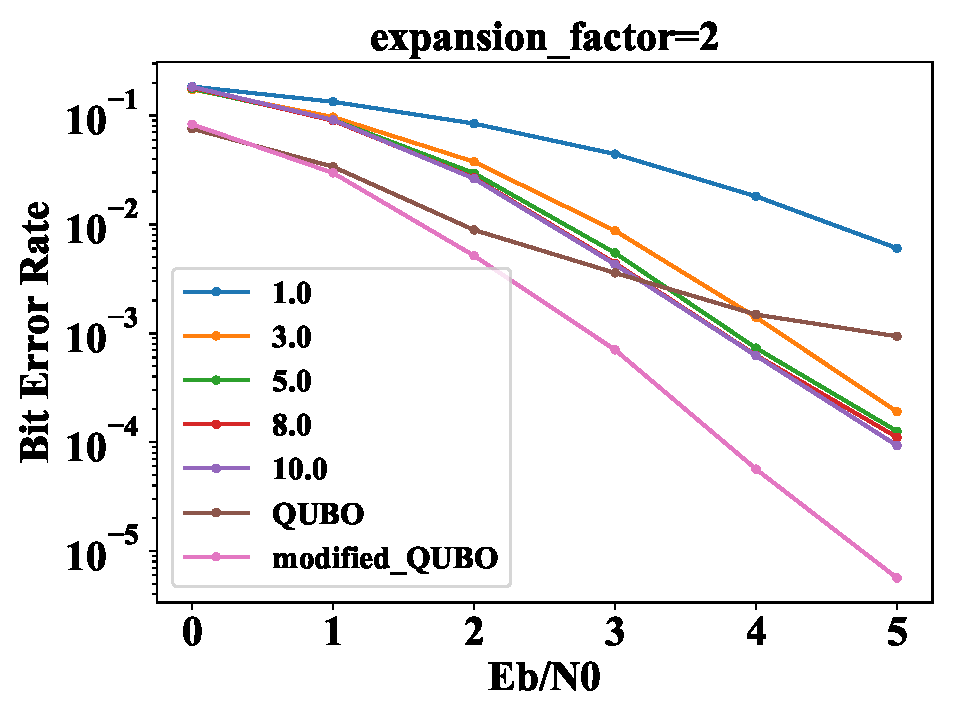
\includegraphics[width=\textwidth]{FIGS/2_.pdf}
  %\caption{This is first figure}
  \end{minipage}%
  \hfill
  \begin{minipage}[b]{.5\textwidth}
  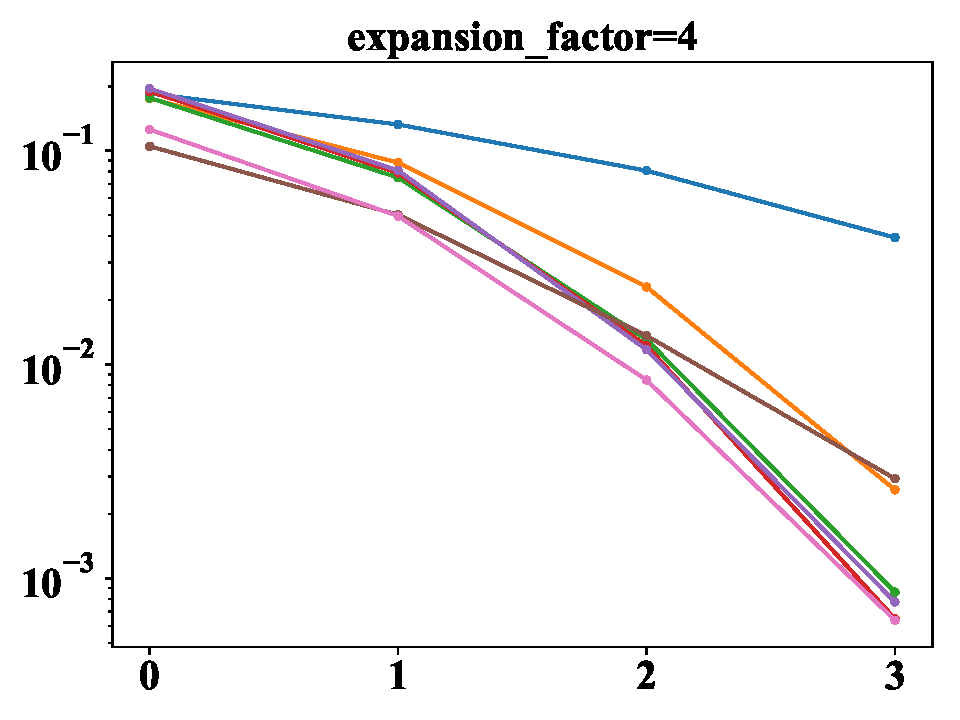
\includegraphics[width = 0.32\textwidth]{FIGS/4_.pdf}
  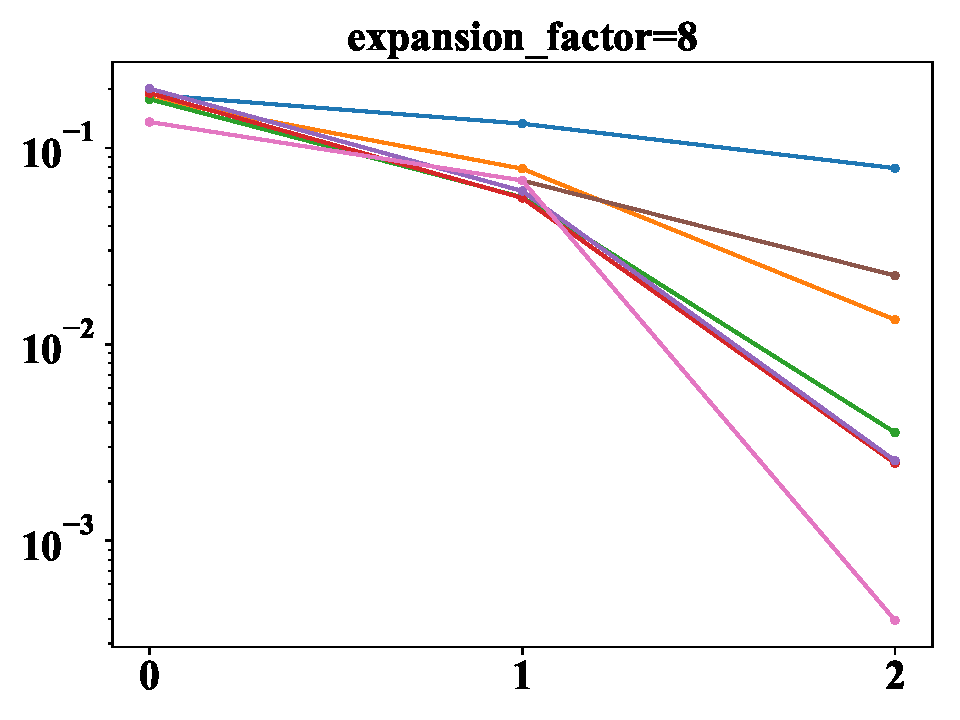
\includegraphics[width = 0.32\textwidth]{FIGS/8_.pdf} 
  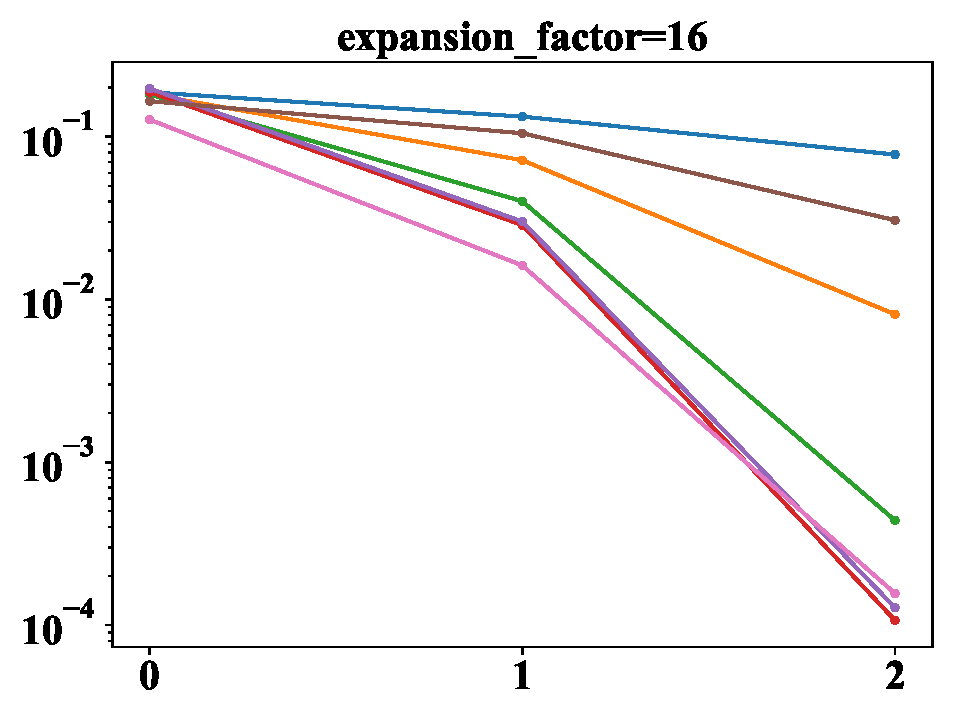
\includegraphics[width = 0.32\textwidth]{FIGS/16_.pdf}
  %\caption{caption}
  \end{minipage} 
  \caption{Bit Error rate achieved by different algorithms at different Signal-noise ratios. Lower the better.}
\label{fig:ber}
\end{figure}

\subsection{Impact of circuit element's noise on solution quality}

\todo{To be implemented}

%\subsection{Circuit Implementation using Cadence}

%\todo{To be implemented}
\end{comment}


\subsection{Comparison with traditional QUBO Formulation }\label{sec:solution_quality}

One thousand messages were encoded using different LDPC codes to obtain the solution quality. These codes were constructed using the 5G-NR standard's base graph 1 with varying expansion factors. The encoded messages were then modulated using BPSK modulation. Noise was added to the modulated signals based on the signal-to-noise ratio (SNR). These corrupted signals were used to test the different algorithms for solution quality. 

Fig.~\ref{fig:ber} shows the solution quality of LDPC decoding using standard QUBO formulations and our proposed formulation (hybrid Ising model or modified QUBO). Since we are analyzing the
quality of the formulation, we use the much faster 
Simulated Annealing (for 10000 iterations) to measure BER. Each message was annealed 10 times with random initializations. Fig.~\ref{fig:ber} shows the average of the bit error rate obtained. We can observe from the graphs that, given the runtime, both the formulations of QUBO yield worse BER compared to our proposed formulation. 

The better performance for our formulation is part of the reason our co-designed
Ising machine performs much better than earlier work using D-Wave annealer.
Additionally, our proposed architecture requires far fewer couplers:
20K couplers (expansion factor 64) vs 
443K and 290K couplers for unary or encoding requires  respectively.

%We find the distinct solutions in these different anneals and rank them according to their Ising energies. Considering this order static, the \textit{expected} Bit Error rate (E(BER($N_a$)))~\cite{kim2019leveraging} for each instance is calculated using the formula~\ref{eqn:expected_ber}.

%\begin{equation}\label{eqn:expected_ber}
%\begin{split}
%E(BER(N_a)) = \sum_{q=1}^{L} \left[ (\sum_{r=q}^{L} P(r))^{N_a} -  (\sum_{r=q+1}^{L} P(r))^{N_a}\right] \\ F(q)/K   
%\end{split}
%\end{equation}
%where K is the number of bits in the message, L is the number of unique solutions obtained by different anneals, r is the rank index of each solution, $P(r)$ is the probability of obtaining the $r_{th}$ solution, $F$ is the number of bit errors in the $q^{th}$ solution, relative to the ground truth and $N_a$ represents number of anneals. The average of 1000 different expected BER is reported as the final Bit Error rate for each SNR. As shown in the figure, modified QUBO gives us the better BER when compared to QUBO formulation.

\begin{figure}[htb]
 \begin{minipage}[b]{.6\columnwidth}
   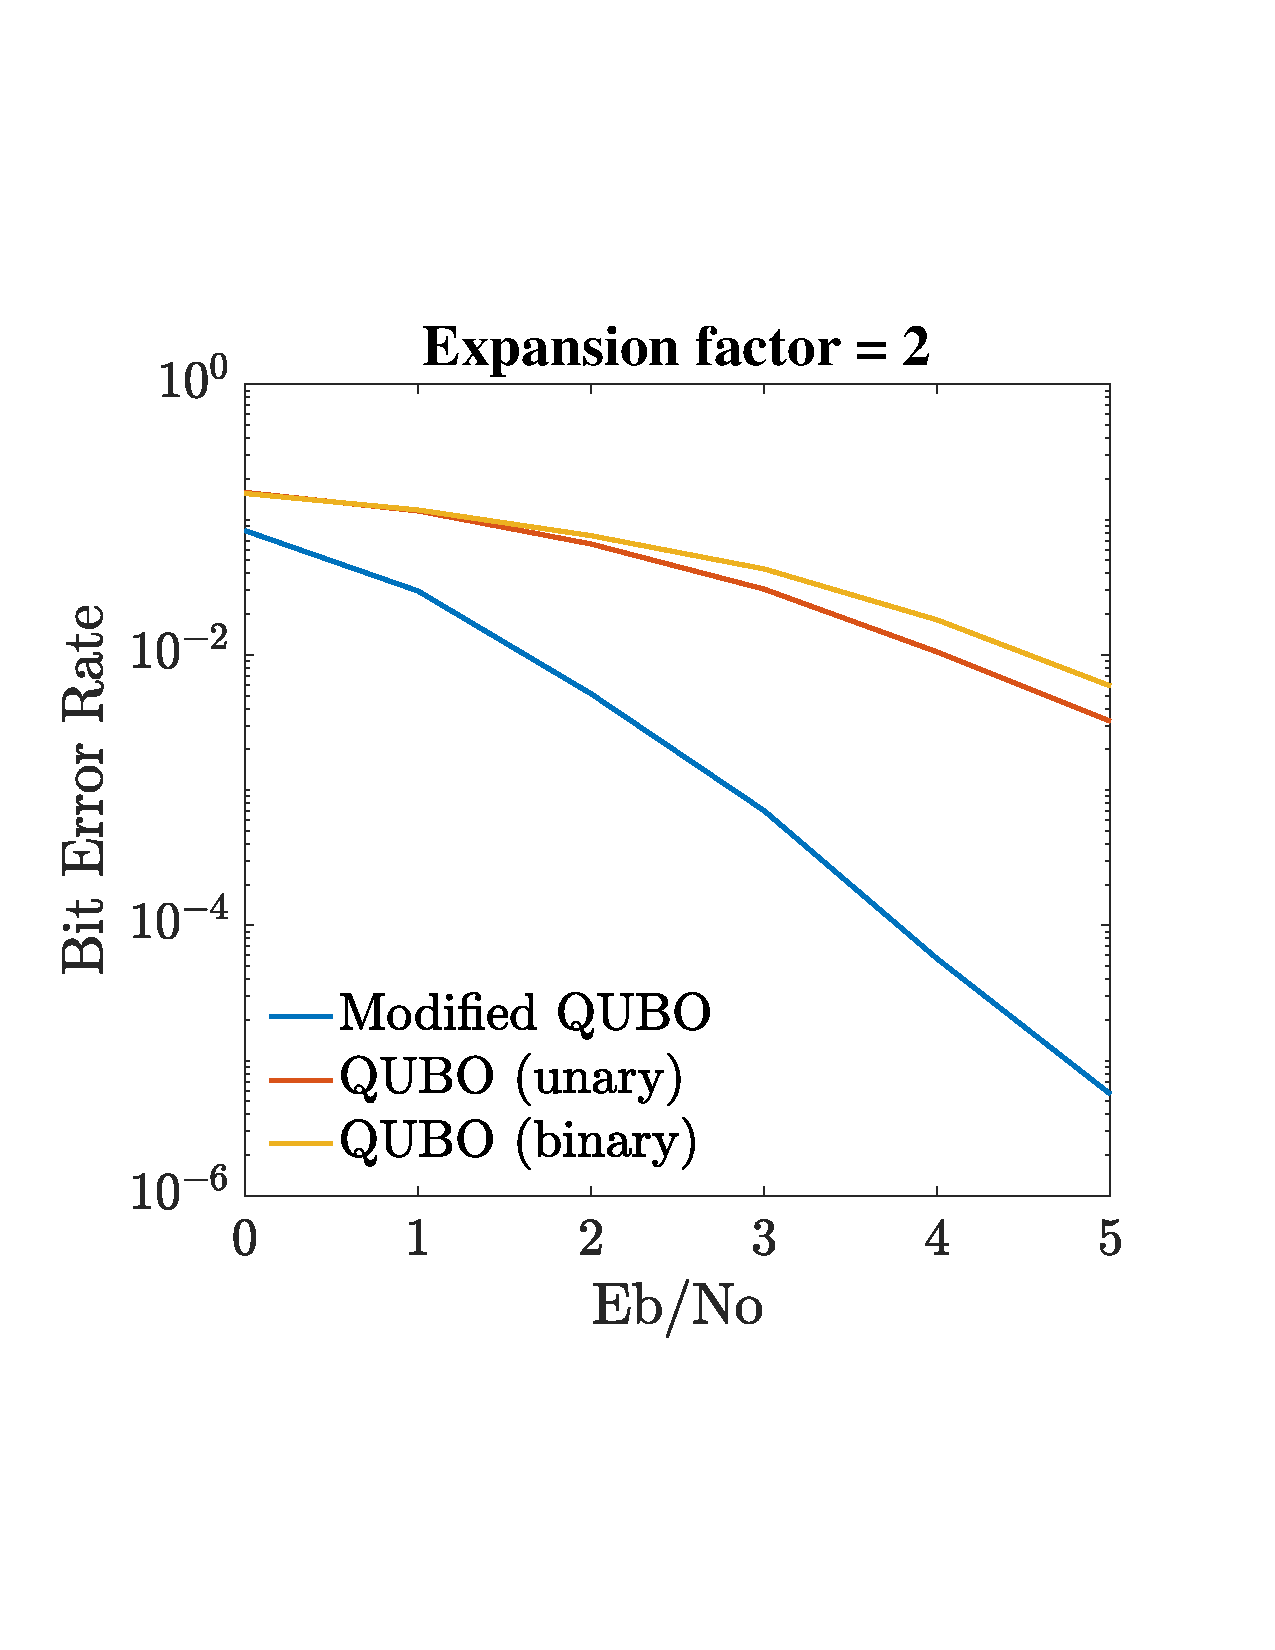
\includegraphics[width =\textwidth]{FIGS/qubo_2.pdf}
  %\caption{This is first figure}
  \end{minipage}%
  \hfill
  \begin{minipage}[b]{.35\columnwidth}
  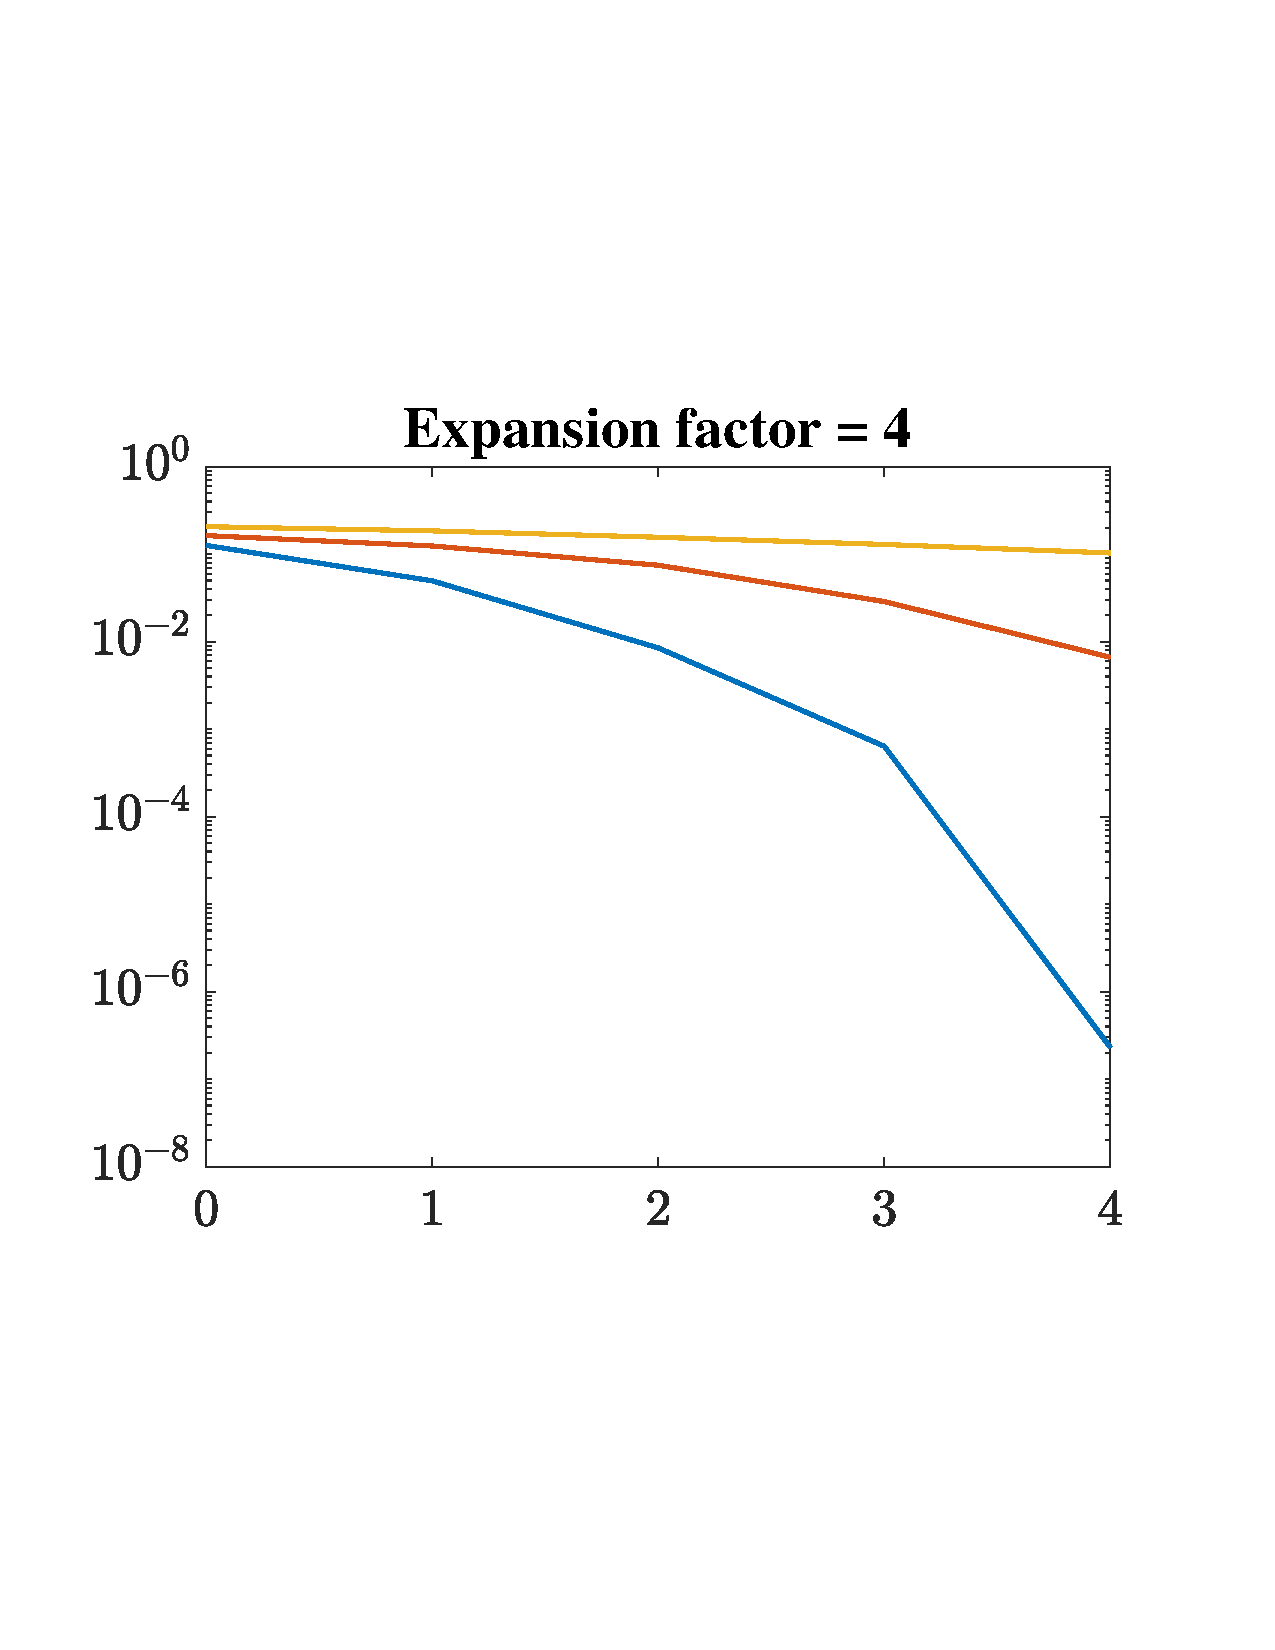
\includegraphics[width = \columnwidth]{FIGS/qubo_4.pdf} 
  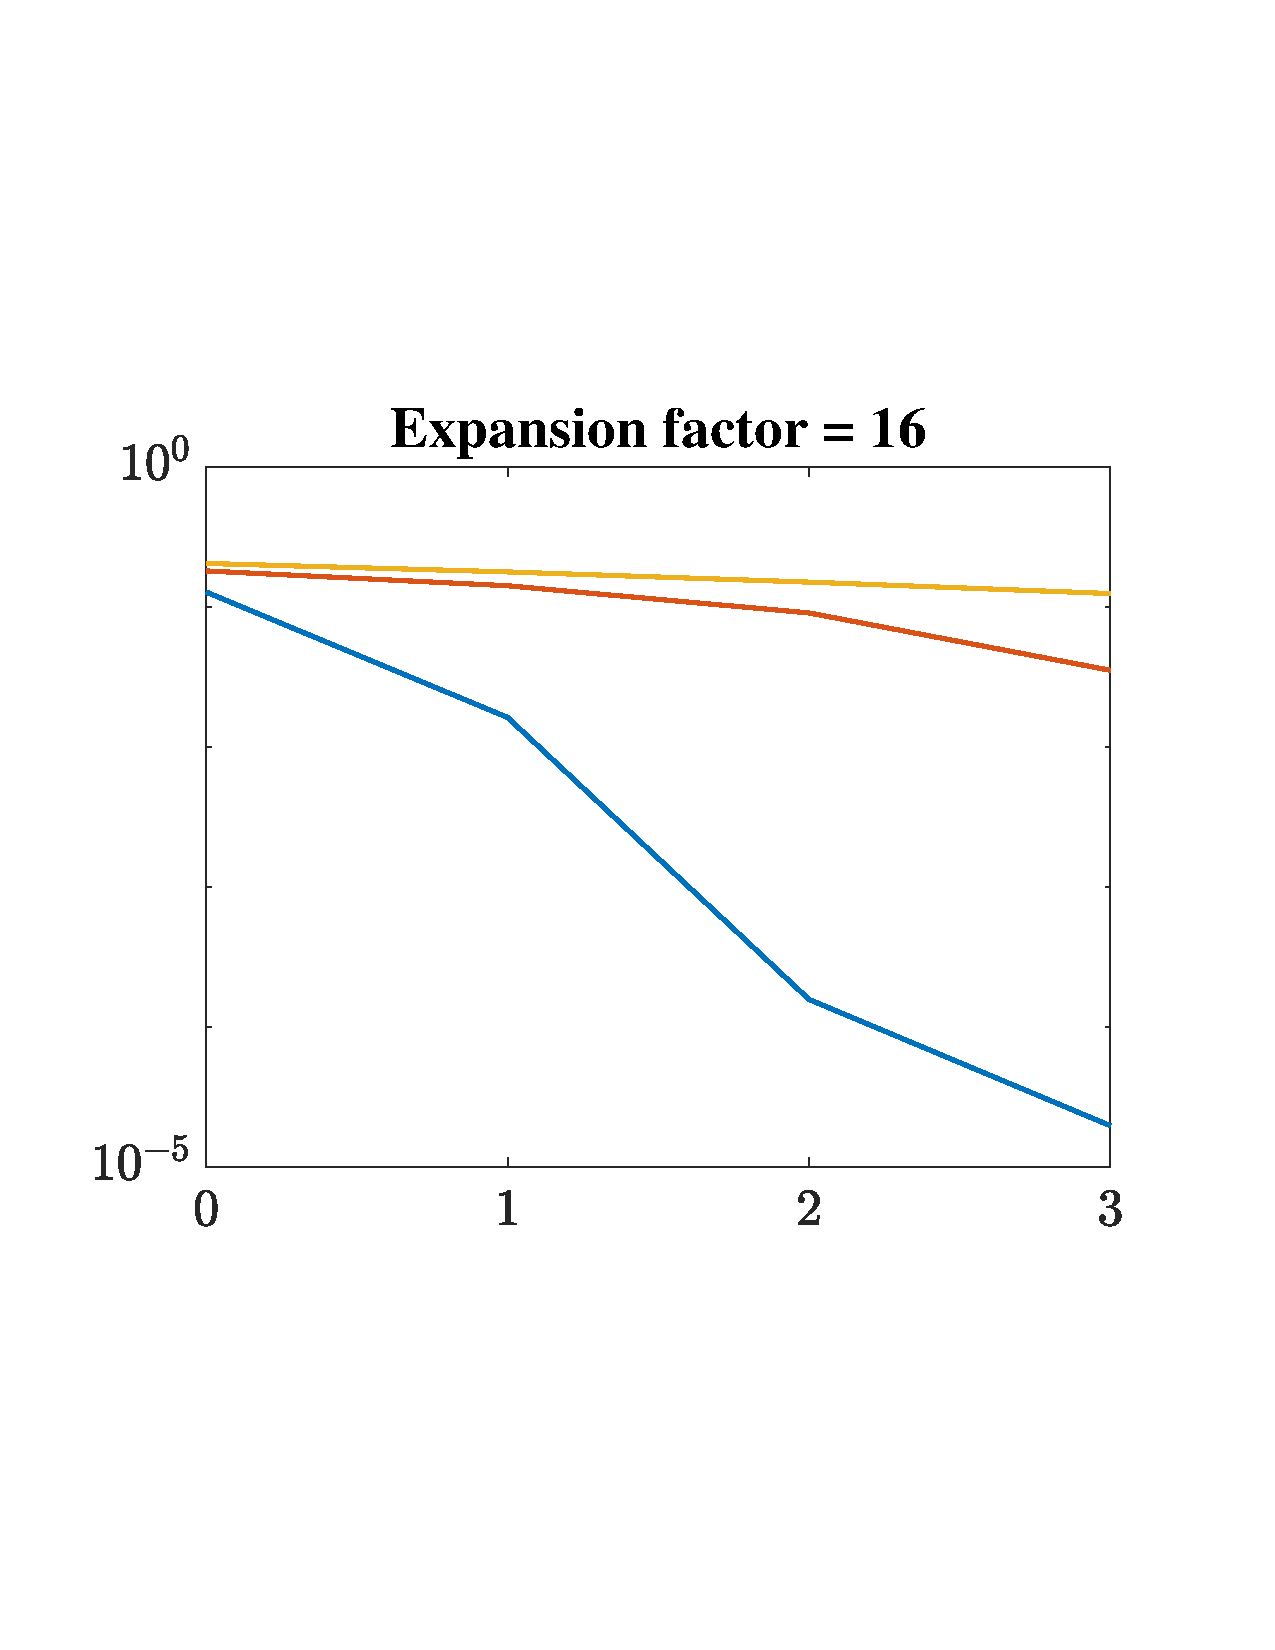
\includegraphics[width = \columnwidth]{FIGS/qubo_16.pdf}
  %\caption{caption}
  \end{minipage} 
  \caption{Bit Error Rate (BER) achieved by different algorithms at different Signal-noise ratios (Eb/No). Lower is better.}
\label{fig:ber}
\end{figure}

\begin{comment}
\begin{figure}[htb]
 \begin{minipage}[b]{.6\columnwidth}
   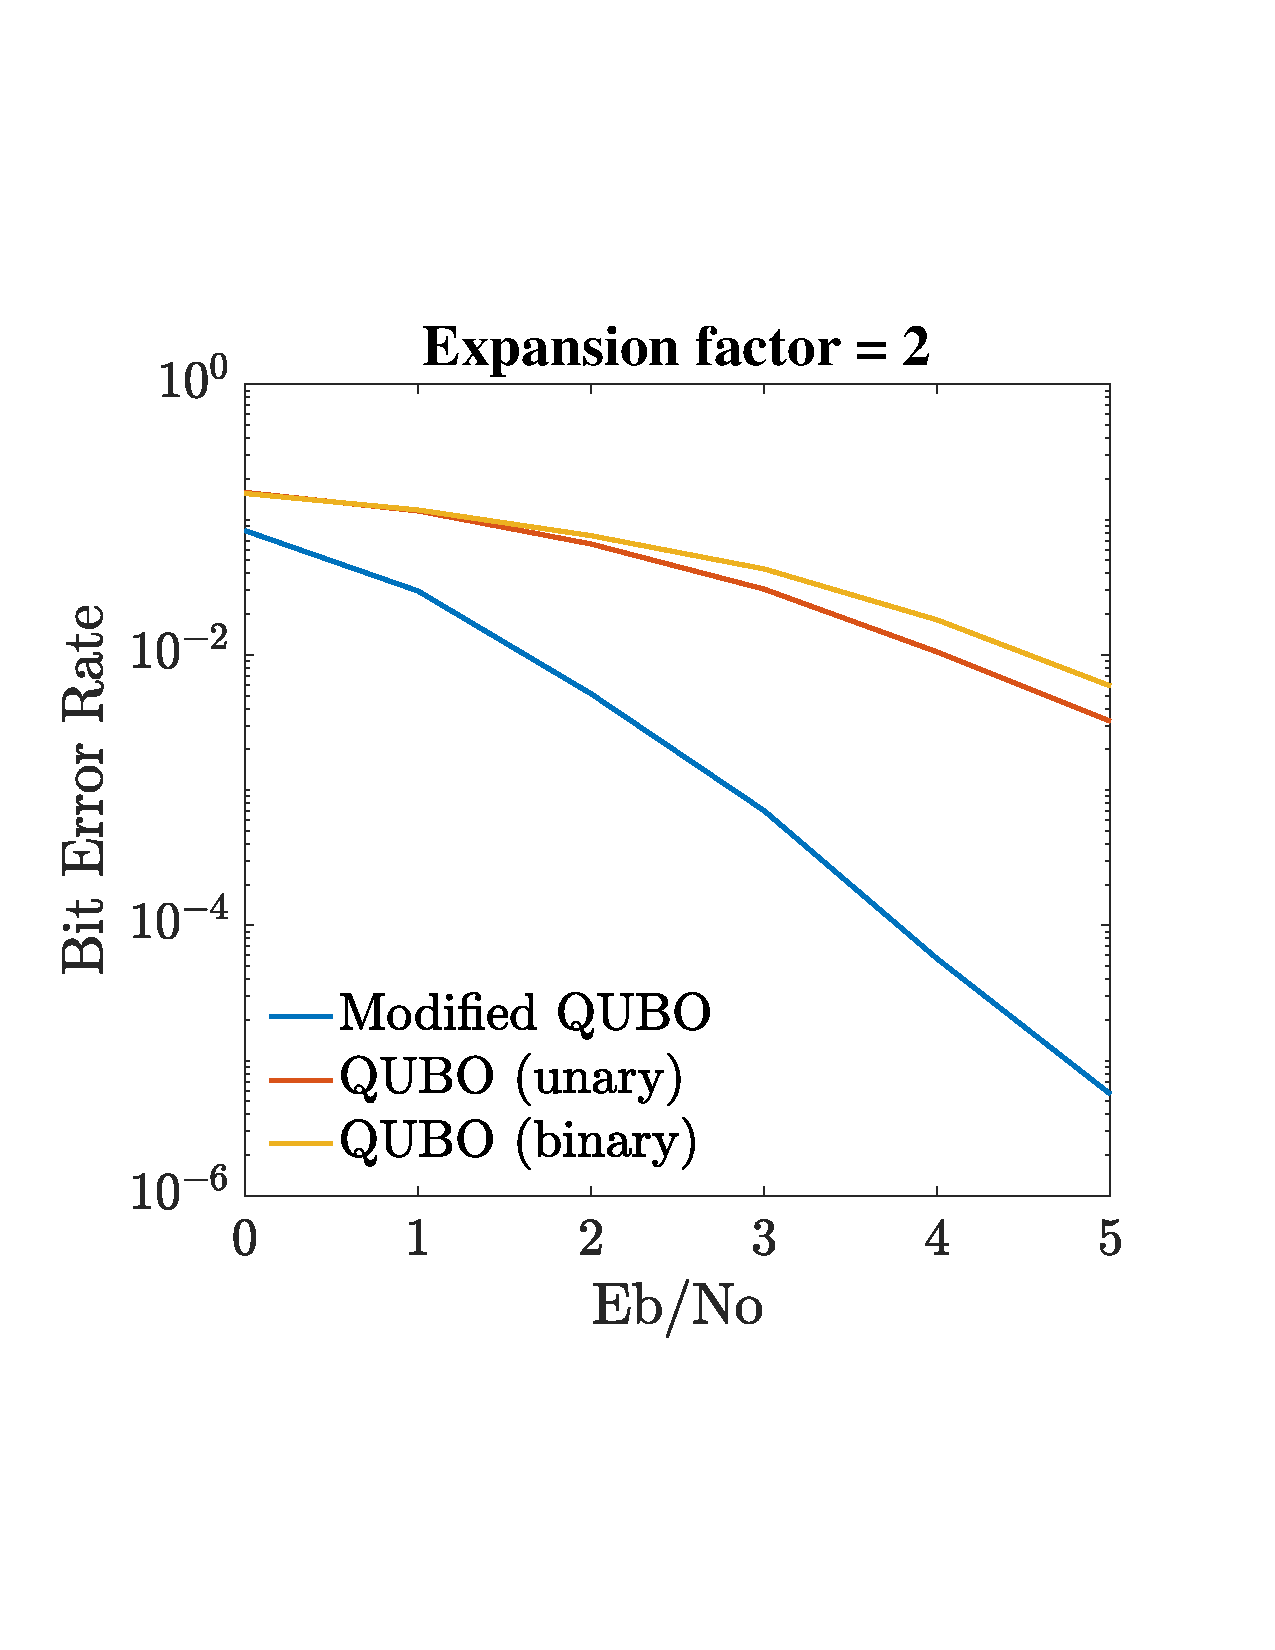
\includegraphics[width =\textwidth]{FIGS/qubo_2.pdf}
  %\caption{This is first figure}
  \end{minipage}%
  \hfill
  \begin{minipage}[b]{.35\columnwidth}
  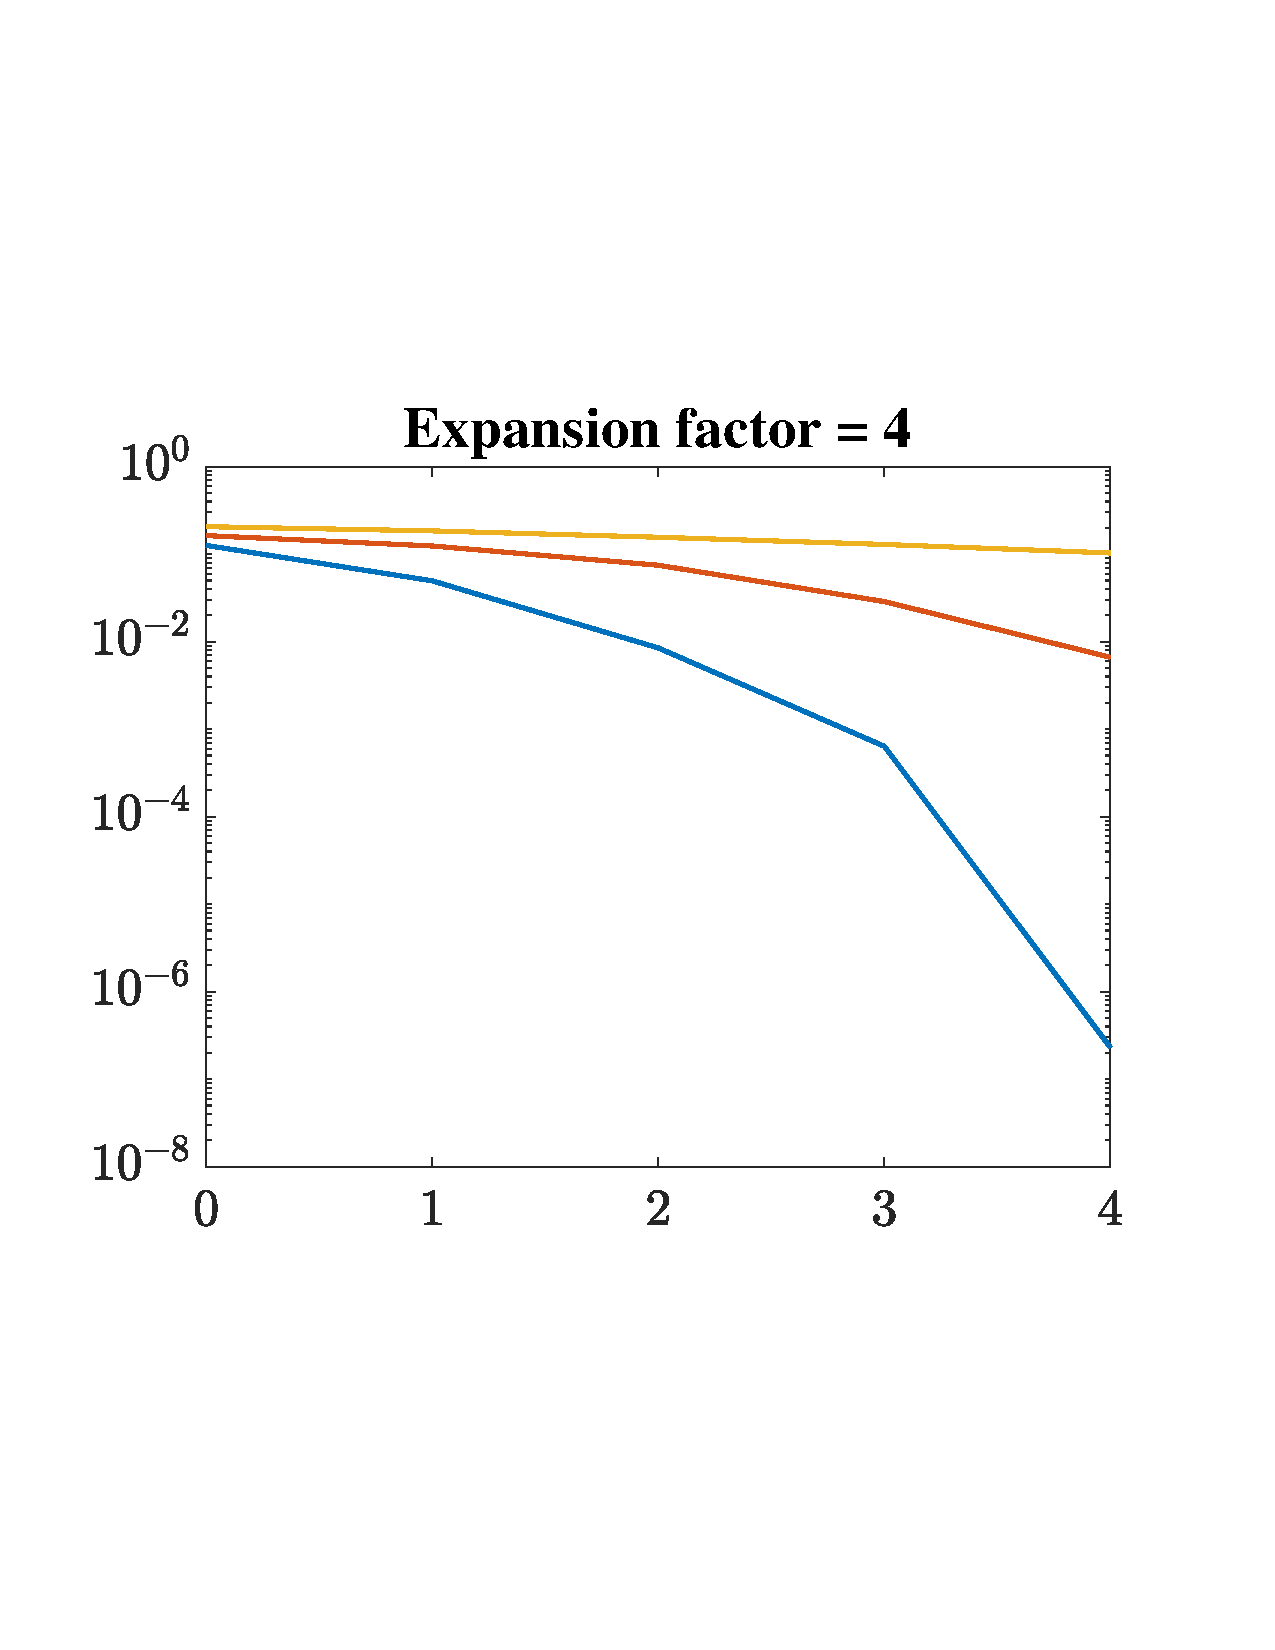
\includegraphics[width = \columnwidth, height=0.72\columnwidth]{FIGS/qubo_4.pdf} 
  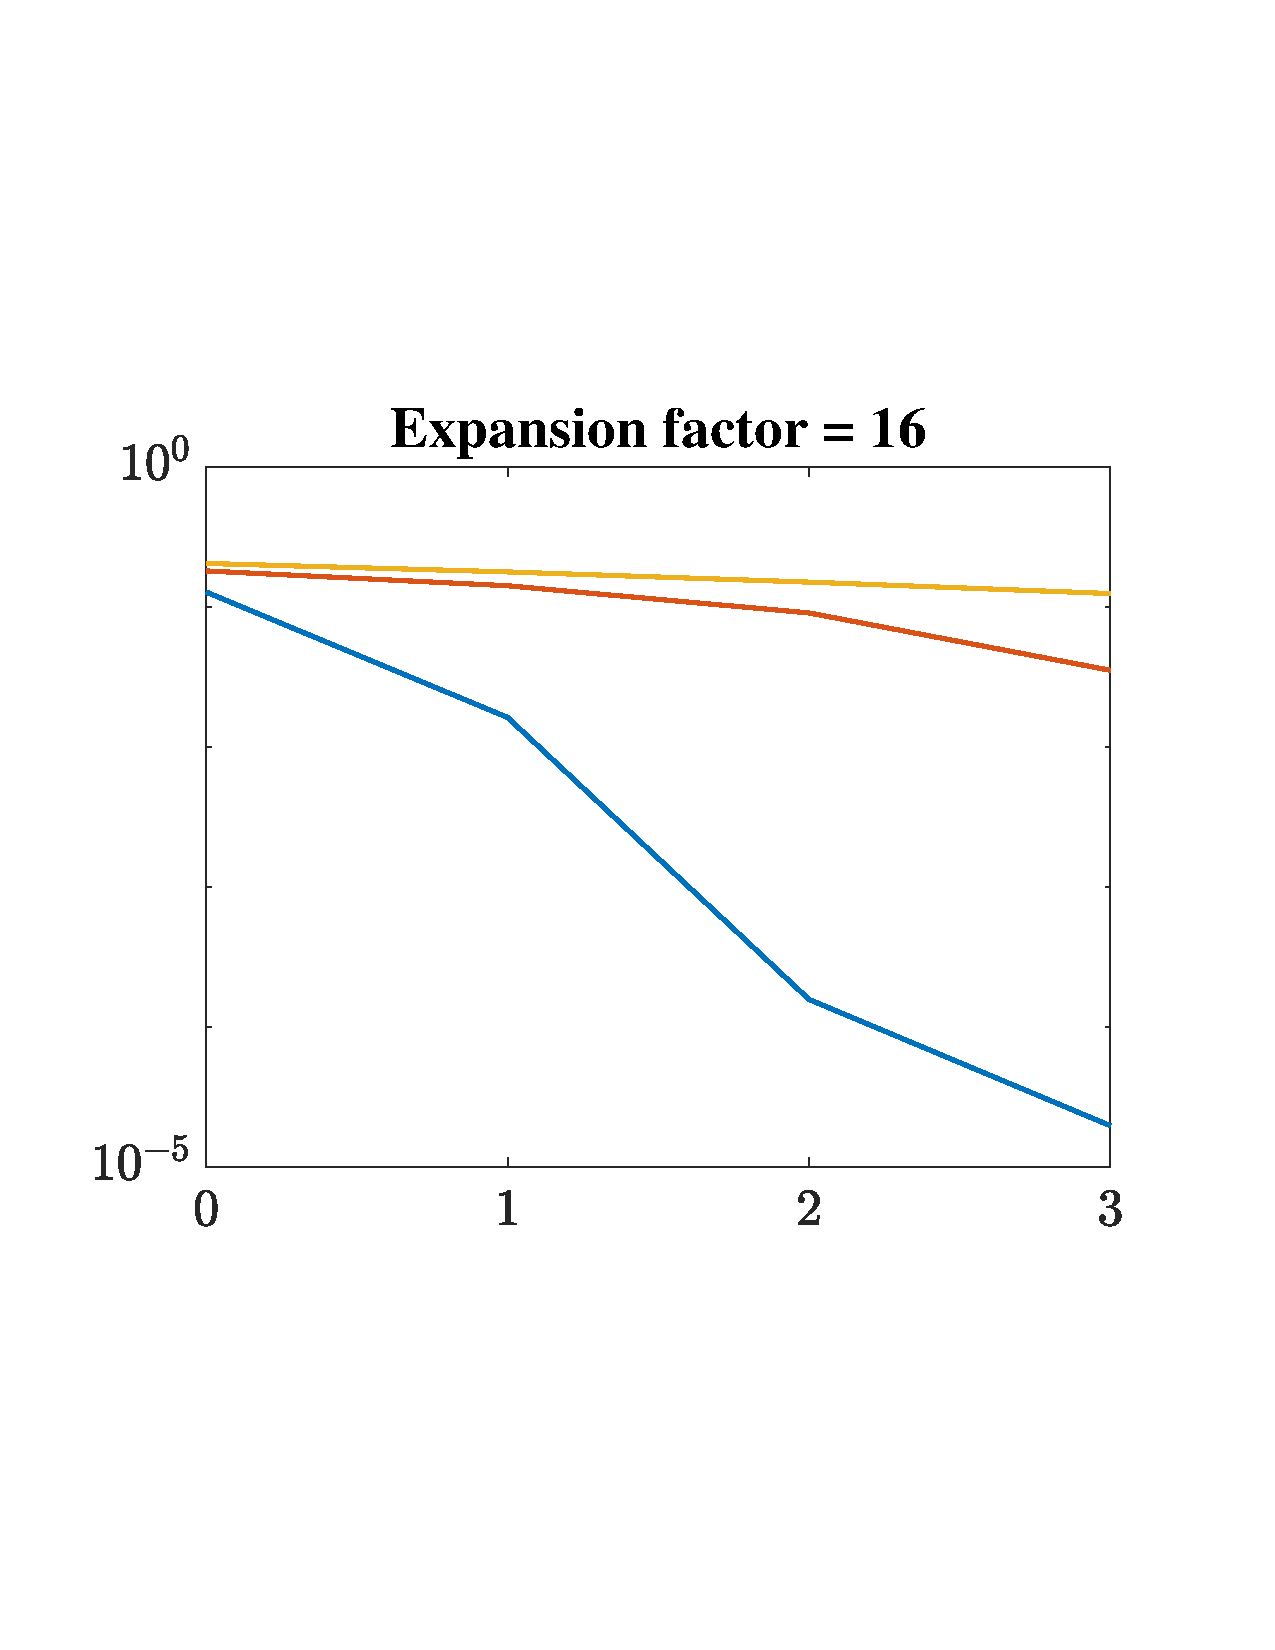
\includegraphics[width = \columnwidth, height=0.72\columnwidth]{FIGS/qubo_16.pdf}
  %\caption{caption}
  \end{minipage} 
  \caption{Bit Error Rate (BER) achieved by different algorithms at different Signal-noise ratios (Eb/No). Lower is better.}
\label{fig:ber}
\end{figure}
\end{comment}

%\todo{needs to be changed}

To compare the solution quality of our proposed design with different variants of belief propagation algorithm, we encoded ten thousand messages using LDPC code constructed using the 5G-NR standard's base graph 1 with an expansion factor of 64. Fig.~\ref{fig:ber_brim} shows the bit error rate obtained by different algorithms. `BP' and `OMS' in the legend represent layered Belief Propagation and layered Offset Min-Sum algorithm, respectively. 
BP and offset Min-sum algorithms were implemented using MATLAB's 5G toolbox. 
We simulate our system evolving for 2.2 $\mu s$. The graph shows that the BER obtained by the hardware approaches the BER rate obtained by BP and its variants at the 7th iteration. 


\begin{figure}[htb]
  \centering
   % 
\includegraphics[width =0.32\textwidth]{LDPC codes/FIGS/ber_sa.pdf}
   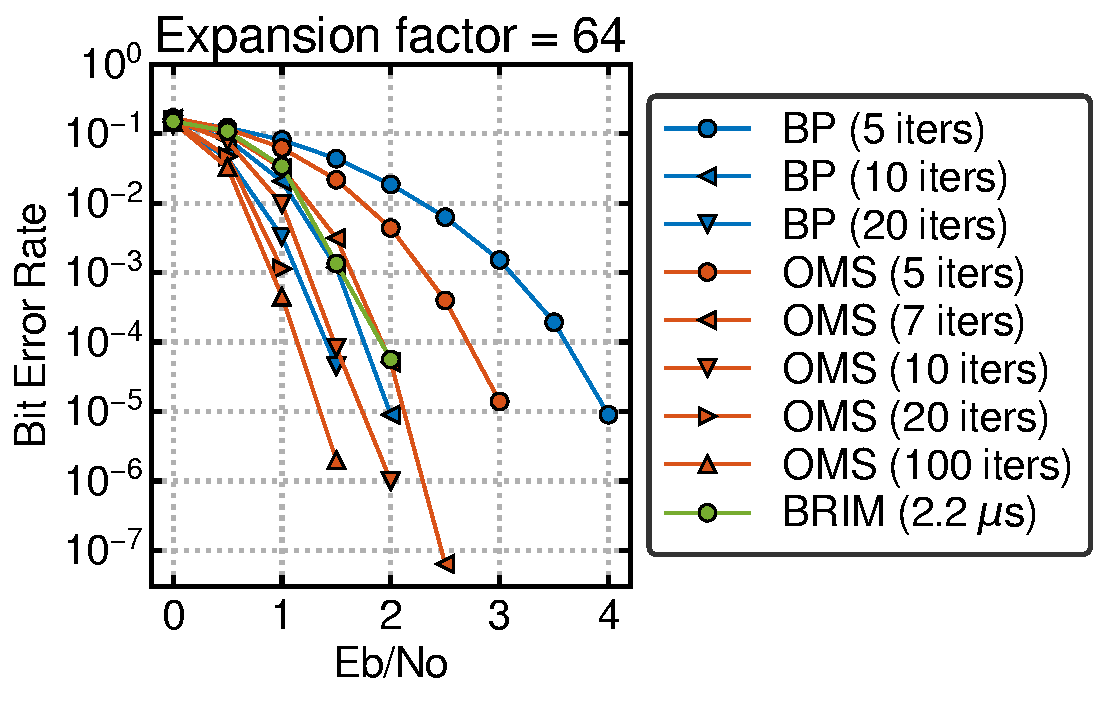
\includegraphics[width=0.50\textwidth]{FIGS/ber.pdf}
  \caption{Bit error rate achieved by different algorithms at different Signal-to-noise ratios. Lower is better.}
\label{fig:ber_brim}
\end{figure}


